\subsection{Problema 4}

\textit {“Se requiere un algoritmo para determinar, de N cantidades, cuántas son de cero, cuántas son menores a cero, y cuántas son mayores a cero.”}

\textbf{Modelo}

El modelo recibe una lista de números y cuenta cuántos son ceros, negativos y positivos. Para ello se definen tres getters que recorren la lista.

\begin{center}
\begin{lstlisting}
int get zeros {
  int count = 0;
  for (int i = 0; i < numbers.length; i++) {
    if (numbers[i] == 0) {
      count++;
    }
  }
  return count;
}

int get negatives {
  int count = 0;
  for (int i = 0; i < numbers.length; i++) {
    if (numbers[i] < 0) {
      count++;
    }
  }
  return count;
}

int get positives {
  int count = 0;
  for (int i = 0; i < numbers.length; i++) {
    if (numbers[i] > 0) {
      count++;
    }
  }
  return count;
}
\end{lstlisting}
\end{center}

Cada getter itera sobre la lista de números y verifica la condición correspondiente, incrementando un contador cuando se cumple.

\textbf{Controlador}

El controlador valida los datos ingresados antes de procesarlos. Primero verifica que se haya ingresado la cantidad de números a procesar.

\begin{center}
\begin{lstlisting}
if (cantidad.isEmpty) {
  String err = "Ingrese la cantidad de números";
  return (0, 0, 0, err);
}

final n = int.tryParse(cantidad);

if (n == null) {
  String err = "Ingrese un valor numérico válido";
  return (0, 0, 0, err);
}

if (n <= 0) {
  String err = "La cantidad debe ser mayor a cero";
  return (0, 0, 0, err);
}
\end{lstlisting}
\end{center}

Luego valida que se hayan ingresado exactamente la cantidad de valores indicada y que todos sean numéricos.

\begin{center}
\begin{lstlisting}
if (valores.length != n) {
  String err = "Debe ingresar exactamente $n números";
  return (0, 0, 0, err);
}

List<double> numeros = [];
for (int i = 0; i < valores.length; i++) {
  if (valores[i].isEmpty) {
    String err = "Complete todos los campos";
    return (0, 0, 0, err);
  }

  final valor = double.tryParse(valores[i]);
  if (valor == null) {
    String err = "Ingrese valores numéricos válidos";
    return (0, 0, 0, err);
  }

  numeros.add(valor);
}
\end{lstlisting}
\end{center}

Finalmente, crea una instancia del modelo y retorna los resultados.

\begin{center}
\begin{lstlisting}
final model = NumbersModel(numeros);
return (model.zeros, model.negatives, model.positives, "");
\end{lstlisting}
\end{center}

\textbf{Vistas}

La vista principal permite ingresar la cantidad de números a procesar. Al presionar el botón de generar campos, se crean dinámicamente los inputs necesarios.

\begin{center}
\begin{lstlisting}
void _actualizarCantidad() {
  final n = int.tryParse(cantidadCtrl.text);
  if (n != null && n > 0 && n <= 20) {
    setState(() {
      cantidad = n;
      valoresCtrl = List.generate(n, (index) => TextEditingController());
      msgErr = "";
    });
  } else if (n != null && n > 20) {
    setState(() {
      msgErr = "La cantidad no puede ser mayor a 20";
      cantidad = 0;
      valoresCtrl = [];
    });
  }
}
\end{lstlisting}
\end{center}

Una vez ingresados todos los valores, se procesan mediante el controlador.

\begin{center}
\begin{lstlisting}
void _calcular() {
  List<String> valores = valoresCtrl.map((c) => c.text).toList();
  final (zeros, negatives, positives, err) = ctrl.procesarNumeros(
    cantidadCtrl.text,
    valores,
  );

  setState(() {
    msgErr = err;
  });

  if (err != "") {
    return;
  }

  Navigator.pushNamed(
    context,
    "/numbers/result",
    arguments: {
      'zeros': zeros,
      'negatives': negatives,
      'positives': positives,
    },
  );
}
\end{lstlisting}
\end{center}

En la pantalla de resultados, se obtienen los argumentos pasados y se muestran en una tarjeta con el conteo de cada categoría.

\begin{center}
\begin{lstlisting}
@override
Widget build(BuildContext context) {
  final args = ModalRoute.of(context)!.settings.arguments as Map<String, int>;

  final int zeros = args['zeros']!;
  final int negatives = args['negatives']!;
  final int positives = args['positives']!;
  final int total = zeros + negatives + positives;
}
\end{lstlisting}
\end{center}

\textbf{Ejecución}

El ejercicio permite ingresar N cantidades y clasifica cada una según su valor. Los resultados muestran cuántos números son cero, menores a cero y mayores a cero.

\begin{figure}[H]
    \centering
    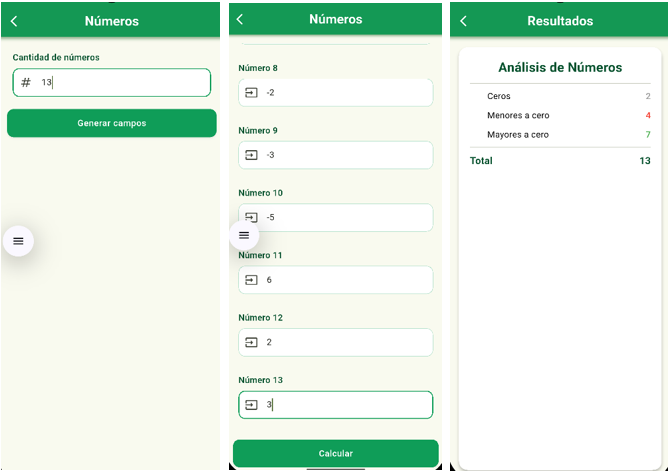
\includegraphics[width=0.8 \textwidth, height=9cm, keepaspectratio]{ejecucion_ej4.png}
    \caption{Ejecución ejercicio 4}
    \label{fig:ej4_ejecuccion}
\end{figure}